\chapter{Organisation du projet}

	\section{Choix des technologies}

		\subsection{Git}

			Nous avons choisi d'utiliser Git comme logiciel de gestion de versions. Quelques-unes des raisons de ce choix sont listées ci-dessous :

			\begin{itemize}
				\item{La gestion des branches est efficace}
				\item{Logiciel de gestion de versions décentralisées, une interruption de service d'un hébergeur n'empêche pas de continuer le travail et il est facile d'héberger son code sur une nouvelle plateforme}
				\item{Meilleure gestion des commits et des conflits que SVN}
			\end{itemize}

			Voici quelques informations supplémentaires concernant notre utilisation de celui-ci.

			\subsubsection{Branches}

				Afin d'utiliser au mieux Git, nous avons fait le choix de créer deux branches "principales". Il s'agit de \textit{master} et de \textit{develop}.\\
				La branche \textit{master} correspond à une version stable qui peut être mise en production. Ainsi, on ne travaillera jamais sur cette branche.\\
				La branche \textit{develop}, quant à elle, est celle à partir de laquelle nous créerons les différentes branches pour le développement de nos fonctionnalités. Ne sont poussées sur celle-ci que les nouvelles fonctionnalités opérationnelles des applications. C'est donc la version en cours de développement.\\
				Les branches créées à partir de \textit{develop} sont les branches correspondant aux fonctionnalités développées, elles commencent toutes par \textit{features/} (correspondant à la modification). Par exemple, pour le développement des fourmis, on créera une branche \textit{features/fourmis}.

			\subsubsection{Nomenclature}

				Nous avons choisi d'établir et d'utiliser une nomenclature pour les messages de commit. Chaque message est préfixé par un mot qui permet d'identifier le type de modification apportée. Nous pouvons par exemple citer l'ajout de fonctionnalités sous le préfixe de \textit{feat}, \textit{fix} pour les corrections de bug, \textit{doc} pour la documentation, etc.

		\subsection{Gradle}

			Gradle est un "build automation system". Il est un équivalent plus récent et plus complet à Maven. Il possède de meilleures performances, un bon support pour de nombreux IDE et permet d'utiliser de nombreux dépôts, dont ceux de Maven, pour télécharger les dépendances dont le projet a besoin. Cet outil se révèle pratique car il automatise complètement la réalisation des tâches usuelles tel que la compilation, l'éxécution et les tests unitaires du code source, etc. Il est également possible de créer ses propres "tasks", afin d'automatiser des actions récurrentes, ou de concevoir et utiliser des plugins pour faciliter la configuration de certains projets (JavaFx11 et plus, Android, ...).

		\subsection{JavaFx}

			Il s'agit d'une technologie plus récente que Swing. De ce fait, beaucoup plus de composants modernes sont disponibles contrairement à Swing. Nous avons fait le choix d'utiliser cette technologie notamment pour élargir nos connaissances sur Java et les librairies usuelles.

	\section{Gestion du projet}

		Afin de faciliter la communication et le bon déroulement de la conception de notre application, divers moyens ont été mis en oeuvre.

		\subsection{GitHub et Forge}

			Bien que nous devions rendre le projet sur la forge, nous avons fait le choix d'utiliser GitHub afin d'héberger et de travailler sur le projet. Ce choix s'est fait au vue de la liste des avantages que cette plateforme apporte :

			\begin{description}
				\item[Webhooks :]{Ils permettent d'obtenir facilement toutes les informations sur ce qui se passe concernant le dépot. Cela est d'autant plus intéressant que Discord permet d'exploiter ces webhooks.}
				\item[Pull Requests :]{Elles permettent de demander une fusion entre deux branches tout en visualisant toutes les mofifications effectuées depuis le dernier commit en commun. Cette fonctionnalité nous a notamment été utile pour effectuer les revues de code.}
				\item[Actions :]{Il est possible d'exécuter certaines actions, par exemple, lorsqu'un évènement se déclenche. Nous avons utilisé cette fonctionnalité afin de lancer automatiquement les tests unitaires à chaque push et pull request. On était alors prévenu dès qu'ils échouaient.}
			\end{description}

			De plus, grâce à git, il suffit simplement d'ajouter une remote vers la forge afin de push les changements sur celle-ci. Cela est d'autant plus pratique que l'entiereté des commits est conservé. Des pushs sur la Forge sont donc réalisés toutes les semaines afin d'actualiser le dépôt. Bien entendu un push final a été effectué sur la Forge pour rendre le projet.

		\subsection{Trello}

			Concernant la répartition et le "listing" du travail à produire, nous avons fait le choix d'utiliser \href{https://trello.com}{Trello}. C'est une plateforme qui nous permet d'utiliser des tableaux pour planifier un projet.

			\begin{figure}[H]
				\centering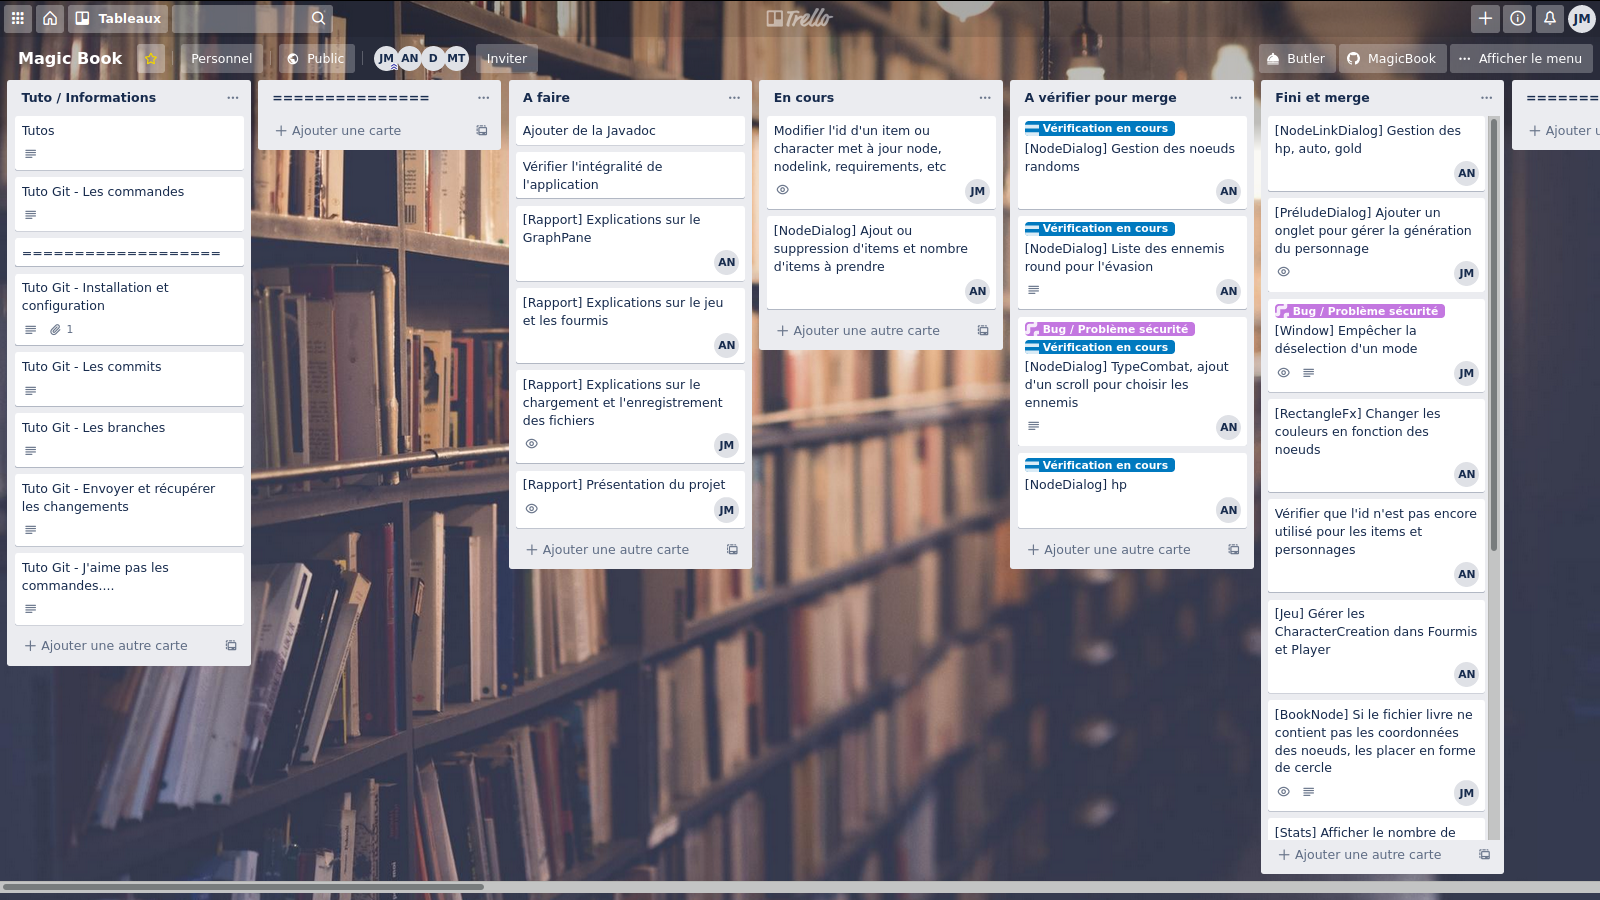
\includegraphics[width=0.64\textwidth, keepaspectratio]{img/trello.png}
				\caption{Notre tableau Trello}
				\label{fig:trello}
			\end{figure}

			Ainsi, comme nous pouvons le constater, les différentes tâches passent par différents états, "\textit{A faire}", "\textit{En cours}", "\textit{A vérifier}", "\textit{Fini et merge}". Enfin, bien que cela ne soit pas visible sur l'image \ref{fig:trello}, il existe un "\textit{Backlog}" sur la droite qui contient les différentes tâches restantes à accomplir. Celles-ci peuvent ensuite être déplacées dans la colonne "\textit{A faire}" au moment où nous jugeons qu'elles peuvent être réalisées.

			Les colonnes "\textit{A verifier}" et "\textit{Fini et merge}" nécessitent quelques précisions. Pour la première, lorsqu'une tâche est terminée, elle est soumise à évaluation et relecture. Cela permet d'obtenir un avis sur la fonctionnalité et d'éviter d'éventuels bugs par la suite mais aussi de garder une cohérence au travers le code. Raisons pour lesquelles les personnes qui effectuent cette relecture sont souvent les mêmes. Enfin, quand celle-ci est vérifiée et validée, on peut alors merge la branche \textit{feature} dans \textit{develop} et ainsi, la déplacer dans la seconde colonne.

		\subsection{Discord}

			Afin de faciliter la communication au sein du groupe, nous utilisons le service de messagerie \href{https://discordapp.com}{Discord} car tous les membres du groupe l'utilisaient déjà de manière personnelle. Celui-ci permet de parler par le biais de "serveurs" gratuits dans lesquels nous pouvons ajouter des salons textuels ou des salons vocaux à volonté. Ainsi, nous avons trois salons de discussion. L'un nommé "\textit{news-magic-book}", qui nous permet d'obtenir toutes les informations sur les push, pull-request, résultats des tests concernant le dépôt sur GitHub. "\textit{important-magic-book}" permet de transmettre des messages importants, sur ce qui a été fait, sur des changements, sur les dates limites concernant le projet, etc. Enfin, "\textit{dev-magic-book}" est une discution beaucoup plus générale dans laquelle on peut demander de l'aide, aider des membres en difficulté, ou même de discuter de certains choix à faire.

			\begin{figure}[H]
				\centering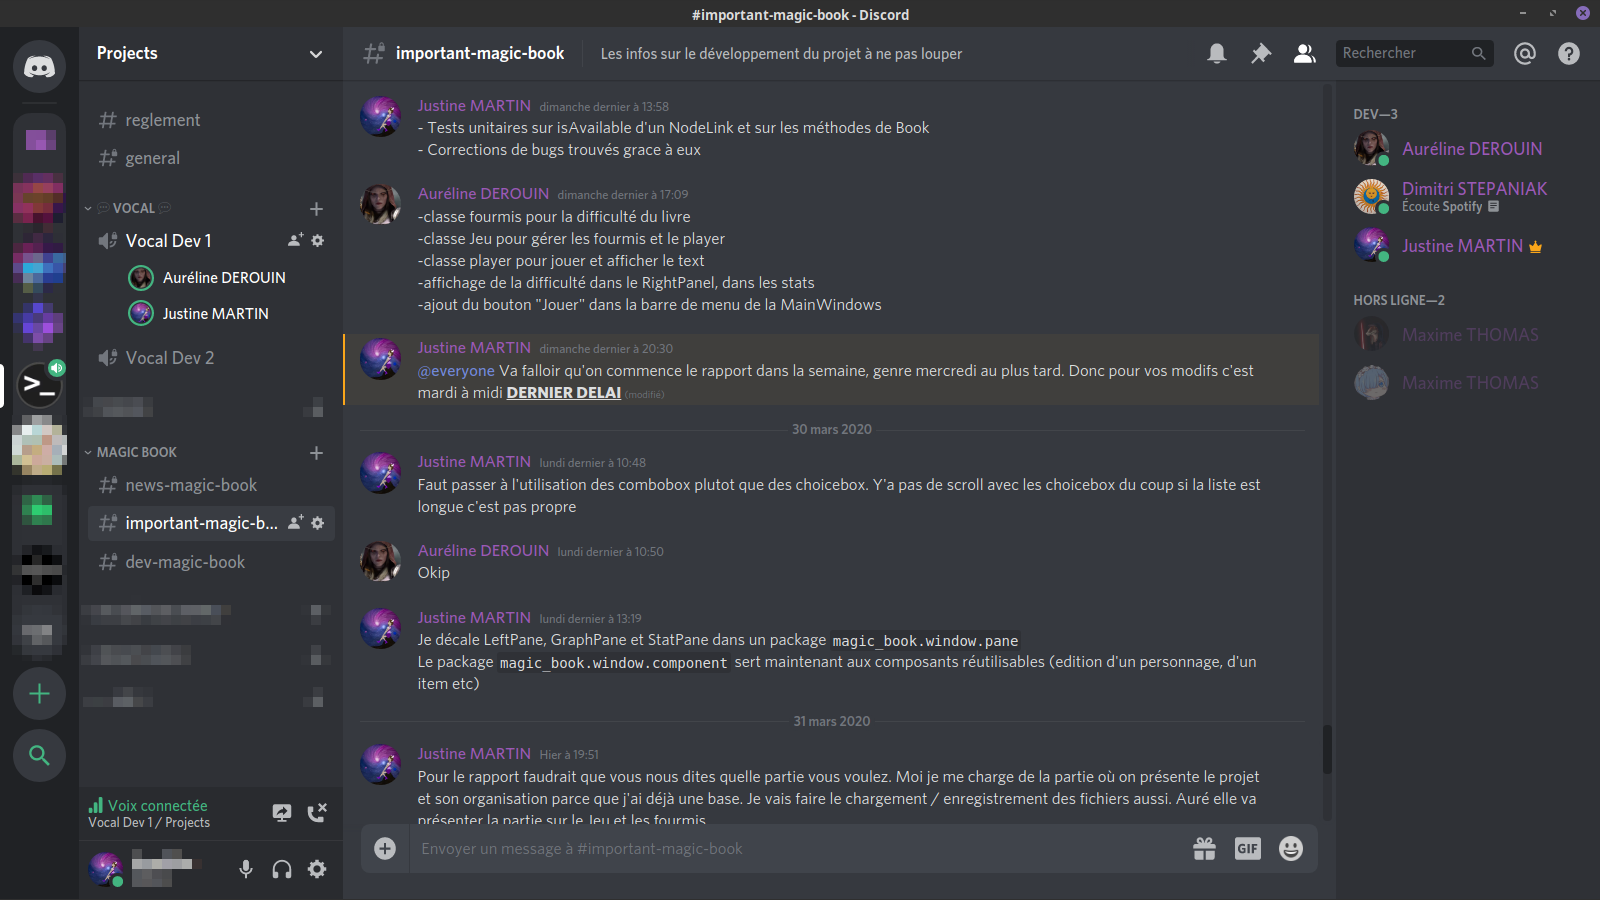
\includegraphics[width=0.64\textwidth, keepaspectratio]{img/discord.png}
				\caption{Notre serveur Discord}
			\end{figure}
